%----------------------------------------------------------------------------
\chapter{Technológia}\label{sect:technológia}
%----------------------------------------------------------------------------

+++ bevezeto a fejezethez +++

%,,,,,,,,,,,,,,,,,,,,,,,,,,,,,,,,,,,,,,,,,,,,,,,,,,,,,,,,,,,,,,,,,,,,,,,,,,,,
\section{Az OpenCV könyvtár}\label{sect:opencv}
%,,,,,,,,,,,,,,,,,,,,,,,,,,,,,,,,,,,,,,,,,,,,,,,,,,,,,,,,,,,,,,,,,,,,,,,,,,,,

Az \textbf{OpenCV}\footnote{\url{http://opencv.willowgarage.com/}} egy nyílt forráskódú gépi látás (computer vision) könyvtár. Elsődleges célja, keretet nyújtani \textbf{valósidejű} képfeldolgozási alkalmazások fejlesztésére. A könyvtár szabadon letölthető és felhasználható a BSD licenc\footnote{\url{http://www.linfo.org/bsdlicense.html}} keretein belül.

\bigskip

Az OpenCV projekt hivatalosan 1999-ben indult az Intel kezdeményezésében. A nagyközönségnek a 2000. évi \textit{,,IEEE Conference on Computer Vision and Pattern Recognition''} konferencián mutatkozott be, majd öt béta-verziót követően 2006-ban jutott el az 1.0-ás hivatalos kiadásig. A fejlesztése itt úgy tűnt, hogy megáll, de végül a projektet a Willow Garage\footnote{\url{http://www.willowgarage.com/}} robotikai kutatólabor vette szárnyai alá. Az ő irányításuk alatt 2008 októberében elkészült az 1.1-es verzióval közel egy időben látott napvilágot az elsõ hivatalos OpenCV-vel foglalkozó könyv \textit{,,Learning OpenCV: Computer Vision with the OpenCV Library''} címmel Gary Bradski és Adrian Kaehler fejlesztõk tollából \cite{opencv_book}. Az egy évvel később, 2009 októberében megjelent 2.0-ás verzióval a projekt nagy fejlődésen esett át. Ebben a verzióban található meg elõször a C++ és Python interfész (ez a meglévő C mellett már három hivatalosan fejlesztett interfészt jelentett), amely az egyszerûbb kezelhetõség, új függvények mellett a meglévő eljárások teljesítmény tekintetében -- különösen többmagos rendszereken -- jobb implementációját kínálta a felhasználóknak.

\bigskip

A projekt életében a következő mérföldkő 2012 augusztusa volt. Ekkor az OpenCV támogatását és fejlesztését az erre a célra alapított \emph{OpenCV.org} non-profit alapítvány vette át. A 2.5-ös verzió kiadásával tovább bővült a támogatott programozási nyelvek listája: innentől már a Java és a MATLAB/OCTAVE is felkerült az elérhető interfészek listájára. Nem hivatalos támogatással, de további wrapper-ek is elérhetők a könyvtárhoz, például C\# vagy Ruby nyelven, ezzel is elősegítve a széleskörű elterjedését. 

Az elmúlt években a GPU-gyorsítás támogatása terén is komoly előrelépésekre került sor. 2010 szeptemberétől érhető el a CUDA, 2012 októberétől pedig az OpenCL interfész.

\bigskip

A fejlesztést különboző platformokra párhuzamosan (cross-platform) történik. Mivel a könyvtár alapvetően a C nyelvre épül, ezért a számos platformon működésre bírható. A dolgozat írásának idején elérhető 2.5-ös stabil verzió a következő operációs rendszerekre elérhető:

\begin{itemize}
  \item asztali (desktop) rendszerek
  \begin{itemize}
    \item Windows
    \item Linux
    \item OS X
    \item OpenBSD
    \item FreeBSD  
  \end{itemize}
  \item mobil operációs rendszerek
  \begin{itemize}
    \item iOS
    \item Android
    \item BlackBerry 10
    \item Maemo
  \end{itemize}   
\end{itemize}

\bigskip

Az OpenCV jelenlegi 2.5-ös verziója elérhető FreeBSD, Linux, Mac OS és Windows operációs rendszerek alá. Széles körben, mondhatni világszerte használt, felhasználói tábora több, mint 40\,000 főt számlál. Köszönhető ez többek között annak, hogy felhasználási lehetőségei igencsak sokrétűek: több, mint 500 optimalizált algoritmust kínál annak érdekében, hogy ,,ne kelljen újra feltalálnunk a kereket''. Sebesség tekintetében érződik a kipróbált, optimalizált algoritmusok használata: az OpenCV a jelenleg elérhető leggyorsabb alternatíva gépi látás terén (\figref{opencv_speed} ábra). Teljesítménye azonban adott esetben még tovább növelhető, mivel ha Intel IPP\footnote{\url{http://software.intel.com/en-us/intel-ipp/}} (Integrated Performance Primitives) támogatást észlel, az abban található szálakra optimalizált algoritmusok használatát fogja preferálni.

\begin{figure}[!ht]
\centering
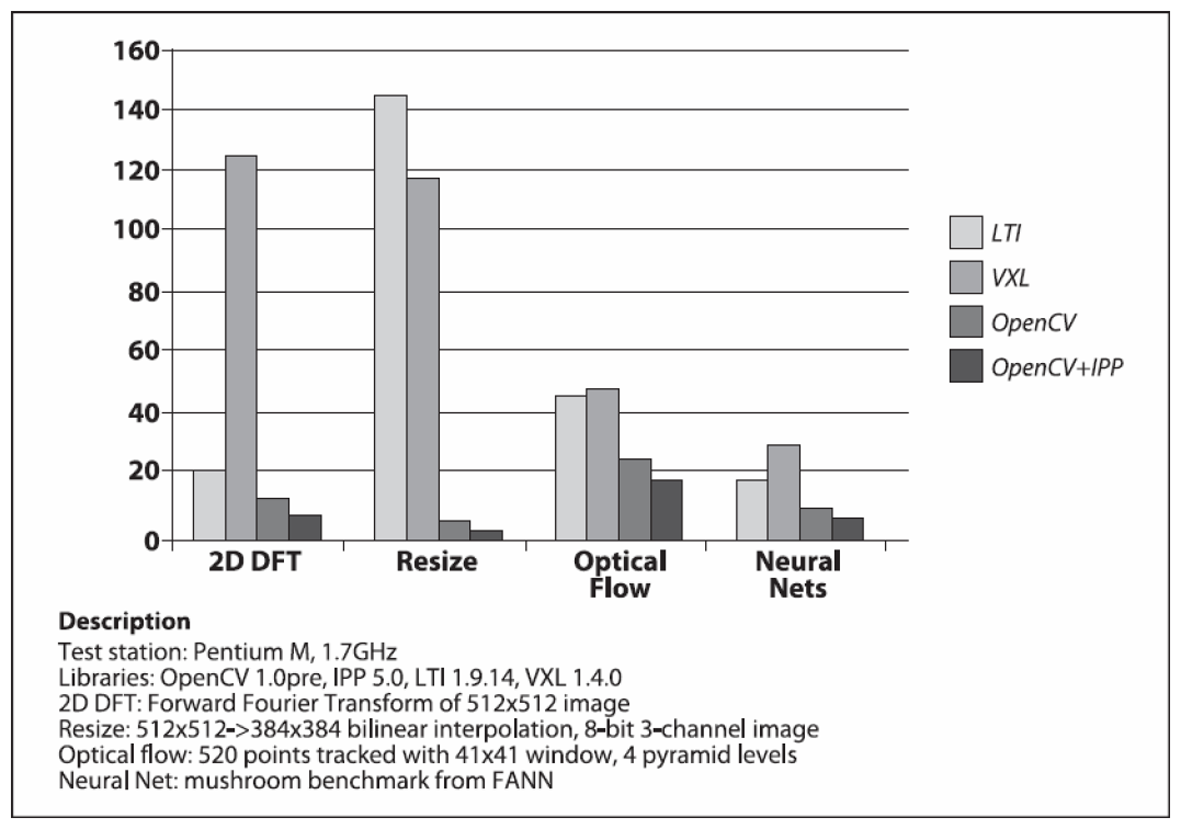
\includegraphics[width=100mm, keepaspectratio]{figures/opencv_speed.png}
\caption{Az OpenCV teljesítménye az LTI és VXL képfeldolgozási könyvtárakkal összehasonlítva.\\Forrás: \cite{opencv_book}}
\label{fig:opencv_speed}
\end{figure}

A teljes funkcionalitás részletekbe menõ bemutatása -- mint láthattuk \cite{opencv_book} -- egy könyvet is megtölt, de a teljesség igénye nélkül tekintsük át, hogy milyen alapvető jellemzői és alkalmazásai vannak a környezetnek:

\begin{itemize}

 \item alap adatstruktúrák
  \begin{itemize}
   \item mátrixok, vektorok
  \end{itemize} 

 \item mátrix és vektor manipuláció, lineáris algebra
  
 \item dinamikus adatstruktúrák
  \begin{itemize}
   \item listák, sorok, halmazok
   \item gráfok és fák
  \end{itemize}

 \item kép és videó input/output
  \begin{itemize}
   \item beolvasás fájlból (kép vagy videó) és kameráról
   \item kiírási lehetőség képként vagy videóként
  \end{itemize}

 \item előfeldolgozás
  \begin{itemize}
   \item él- és sarokkeresés
   \item mintavételezés és interpoláció
   \item színkonverzió
   \item morfológiai operátorok
  \end{itemize}

 \item struktúraanalízis
  \begin{itemize}
   \item távolság- és Hough-transzformáció
   \item kontúrfeldolgozás
   \item sablonillesztés
   \item különböző momentumok
   \item Delaunay háromszögelés
  \end{itemize}

 \item kamerakalibráció
  \begin{itemize}
   \item kalibrációs mintázatok felismerése és követése
   \item fundamentális mátrix becslés
   \item homográfia becslés
   \item sztereó megfeleltetés
  \end{itemize}
  
 \item mozgásanalízis
  \begin{itemize}
   \item optical flow
   \item mozgásszegmentálás és -követés
  \end{itemize}

 \item objektumfelismerés
  \begin{itemize}
   \item eigen-módszerek
   \item rejtett Markov-modell (Hidden Markov Model -- HMM)
  \end{itemize}
  
 \item GUI és rajzolás
  \begin{itemize}
   \item kép és videó megjelenítés
   \item billentyűzet és egérkezelés
   \item egyenes, kör, poligon, szöveg rajzolása
  \end{itemize}
  
\end{itemize}

Láthatjuk, hogy a fent felsorolt funkciókkal a gépi látás terén rengeteg egyszerűbb feladatot szinte ,,egy lépésben'', beépített, optimalizált eljárások segítségével oldhatunk meg. Ha nagyobb szabású projektbe kezdünk, akkor is hasznunkra lehet, hogy részben vagy egészében egy több tízezres felhasználói tábor (melynek jelentős részét aktív kutatók alkotják) visszajelzései alapján fejlesztett környezetre építhetjük munkánkat.

Az OpenCV régebbi verzióiban a számos előny mellett hátrányként volt megemlíthető, hogy segítségével a felhasználói felületet csak nagyon leegyszerűsített módon szabhattuk testre. Igaz, hogy a könyvtár feladata elsősorban a képfeldolgozás és nem a megjelenítés, így ebből a nézőpontból a beépített kép és videó megjelenítési lehetőség, billentyűzet- és egérkezelés valamint trackbarok (csúsztatható kezelőszerv értékek beállítására) létrehozásának lehetősége inkább hozzáadott értékként jelent meg, azonban ez nem változtat azon a tényen, hogy ha igény van felhasználóbarát kezelőfelület készítésére, az OpenCV-t mindenképpen integrálnunk kellett valamely elterjedt grafikus felhasználói felület toolkittel.

\bigskip

A X.X verziótól kezdődően megjelent egy némileg fejlettebb Qt alapú felhasználói felület. Teljes szabadságot még ez sem ad a felületek kialakításában, de az egyszerűbb projektek kezelőszerveinek és megjelenítésének problémája már kielégítően elvégezhető egyéb eszköz használata nélkül.

%,,,,,,,,,,,,,,,,,,,,,,,,,,,,,,,,,,,,,,,,,,,,,,,,,,,,,,,,,,,,,,,,,,,,,,,,,,,,
\section{A Qt keretrendszer}\label{sect:qt}
%,,,,,,,,,,,,,,,,,,,,,,,,,,,,,,,,,,,,,,,,,,,,,,,,,,,,,,,,,,,,,,,,,,,,,,,,,,,,

A \textbf{Qt} (ejtsd az angol ,,cute'' szó mintájára: kjút) keretrendszer egy széles körben használt szoftver, amelyet egyrész grafikus felhasználói felületek (Graphical User Interface -- GUI), másrészt parancssoros (Command Line Interface -- CLI) alkalmazások feljesztésére is használnak. A grafikus felhasználói felületek fejlesztése során a Qt úgynevezett wiget-toolkitként funkcionál -- kis, önálló elemek (widgetek) felhasználását és összekötését teszi lehetővé, ezek összességéből áll össze az elkészült grafikus felület. A szoftver a  GPL~v3\footnote{TODO} illetve LGPL~v2\footnote{TODO} licencek szerint szabadon elérhető.

A keretrendszer egyik nagy előnyének számít más rendszerekkel összehasonlítva, hogy a grafikus felületek kirajzolásakor minden operációs rendszeren igyekszik az elérhető natív elemeket használni, ennek köszönhetően (a natív kirajzolásokból származó nagyszerű performancia mellett) a Qt-vel fejlesztett alkalmazások semmelyik platformon nem tűnnek rendszeridegennek.

\bigskip

A Qt projekt első hivatalos kiadása a Nokia \emph{Qt Development Frameworks} csoport égisze alatt látta meg a napvilágot, miután a finn mobilgyártó felvásárolta a technológiát a norvég Trolltech vállalattól. Ennek megfelelően a kezeti években az asztali platformok mellett leginkább a Symbian operációs rendszer támogatása jelentette a fő csapásirányt. A Nokia azonban 2011-ben szakított saját fejlesztésű operárciós rendszerével, és a további bizalmát a Microsoft akkori és elkövetkező mobilplatformjaiba (Windows Phone 7, majd 8) fektette.

Ezt követően a Nokia megvált a rendszer jogaitól, és azok a Digia\footnote{TODO} vállalathoz kerültek, amely azóta is a projekt fejlesztője és karbantartója. A tranzakció után az új tulajdonos közvetlen célnak túzte ki, hogy aktualizálják a Qt által támogatott platformok listáját az időközben népszerűvé vált rendszerekkel.

A dolgozat írásakor támogatott fontosabb operációs rendszerek:

\begin{itemize}
  \item Windows (XP és 7)
  \item OS X
  \item Linux, FreeBSD, OpenBSD
  \item iOS
  \item Android
  \item QNX (BlackBerry 10)
\end{itemize}

\bigskip

A Qt-ot használó alkalmazások programozási nyelve alapvetően a sztenderd C++, a \emph{Meta Object Compiler} (moc) kódgenerátorral kiegészítve, amely számos beépített makróval teszi könnyebbé a fejlesztést. Több más programozási nyelv is használható az ún. kötések (bindings) használatával. A Qt 4-es verziójához elérhető kötések listája a teljesség igénye nélkül:

\begin{itemize}
  \item TODO
  \item TODO
  \item TODO
\end{itemize}

\bigskip

A Qt 4-es verziója nagyjából 6 éven át 

%,,,,,,,,,,,,,,,,,,,,,,,,,,,,,,,,,,,,,,,,,,,,,,,,,,,,,,,,,,,,,,,,,,,,,,,,,,,,
\section{Módosított kamera}\label{sect:infracam}
%,,,,,,,,,,,,,,,,,,,,,,,,,,,,,,,,,,,,,,,,,,,,,,,,,,,,,,,,,,,,,,,,,,,,,,,,,,,,

+++ kamera infok, LED csere, fenykep +++